\section{The Chinese Wall Security Policy}

The first security models that emerged were mainly concerned with military, and were thus tailored to fit the needs of the military. 
In \cite{brewer1989chinese} a model that is relevant for commercial applications is presented.
This model fits the needs of corporate business services like an analyst that must uphold the confidentiality of his clients, meaning that he cannot advise a corporation if he has insider knowledge of a competitor. \cite{brewer1989chinese}

\subsection*{The Chinese Wall Model}
A Chinese wall is defined as the separation between what can be accessed and what cannot be accessed by a user of the system.
Information is stored in a hierarchy with three levels. 
This hierarchy is depicted on \cref{hierarchy}

\begin{figure}
	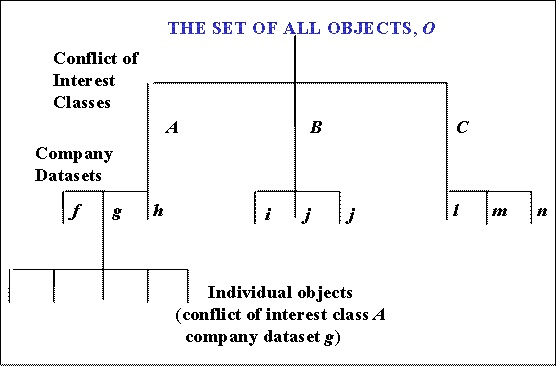
\includegraphics[width=0.6\textwidth]{chinesewall}
	\caption{The hierarchy of the Chinese Wall model. (evt ref til \url{https://www.jpo.go.jp/shiryou/s_sonota/hyoujun_gijutsu/info_sec_tech/c-2-2.html})}
	\label{hierarchy}
\end{figure}

\begin{itemize}
	\item The lowest level contains individual items of information, stored in objects.
	\item The middle level contains company datasets that group all information that concern one company. 
	\item The highest level contains conflict of interest classes which group companies that are in competition.
\end{itemize}

\paragraph{Example} A conflict class could be \emph{Oil companies} which contains \emph{Statoil} and \emph{Shell}. \emph{Statoil} contains objects of information that could compromise the company if \emph{Shell} would obtain the information.


\subsection{The Security Policy}
The concept of the Chinese wall security policy is that a \principal that has access to information about company A which resides in a conflict of interest class C cannot access information about company B if B is conflict of interest class C.
This policy is being upheld by two properties, the \emph{simple security} property and the \emph{star property} corresponding to the identical properties defined in Bell Lapadula \stefan{ref til definitionen i Bellapadula}.

\paragraph{Simple Security}

When a subject S requests to read an object O, this can only be permitted if one of the following requirements are fulfilled:

\begin{itemize}
\item O is in the same company dataset as an object already accessed by S (the object is within the wall)
\item O belongs to a entirely different interest class C than S has previously accessed
\end{itemize}



*-Property
